\documentclass[border=10pt]{standalone}
\usepackage{tikz}\usepackage{amsmath}\usetikzlibrary{arrows.meta}
\begin{document}
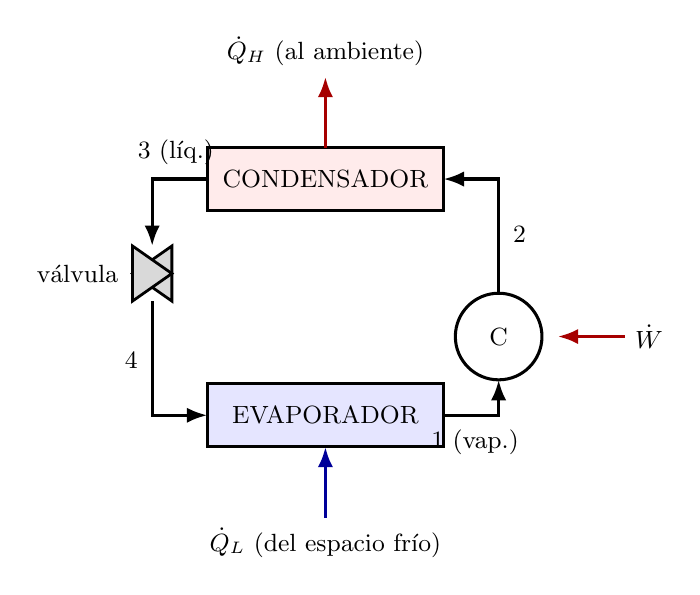
\begin{tikzpicture}[line width=1pt,>={Latex[length=2.6mm]}]
  % condensador (arriba, cede Q_H)
  \fill[red!8] (1.5,3.0) rectangle (4.5,3.8); \draw[line width=1.1pt] (1.5,3.0) rectangle (4.5,3.8);
  \node at (3.0,3.4){\small CONDENSADOR};
  % evaporador (abajo, absorbe Q_L)
  \fill[blue!10] (1.5,0) rectangle (4.5,0.8); \draw[line width=1.1pt] (1.5,0) rectangle (4.5,0.8);
  \node at (3.0,0.4){\small EVAPORADOR};
  % compresor (derecha)
  \draw[line width=1.1pt] (5.2,1.4) circle (0.55); \node at (5.2,1.4){\small C};
  % valvula (izquierda)
  \fill[black!15] (0.55,2.2)--(1.05,2.55)--(1.05,1.85)--cycle; \draw[line width=1.0pt] (0.55,2.2)--(1.05,2.55)--(1.05,1.85)--cycle;
  \fill[black!15] (1.05,2.2)--(0.55,2.55)--(0.55,1.85)--cycle; \draw[line width=1.0pt] (1.05,2.2)--(0.55,2.55)--(0.55,1.85)--cycle;
  \node[left] at (0.5,2.2){\small válvula};
  % tuberias (sentido: evap->compr->cond->valv->evap)
  \draw[->,line width=1.2pt] (4.5,0.4)--(5.2,0.4)--(5.2,0.85); \node[below] at (4.9,0.35){\small 1 (vap.)};
  \draw[->,line width=1.2pt] (5.2,1.95)--(5.2,3.4)--(4.5,3.4); \node[right] at (5.25,2.7){\small 2};
  \draw[->,line width=1.2pt] (1.5,3.4)--(0.8,3.4)--(0.8,2.55); \node[above] at (1.1,3.45){\small 3 (líq.)};
  \draw[->,line width=1.2pt] (0.8,1.85)--(0.8,0.4)--(1.5,0.4); \node[left] at (0.75,1.1){\small 4};
  % interacciones
  \draw[->,red!65!black,line width=1.3pt] (3.0,3.8)--(3.0,4.7); \node[above] at (3.0,4.7){\small $\dot Q_H$ (al ambiente)};
  \draw[->,blue!60!black,line width=1.3pt] (3.0,-0.9)--(3.0,0); \node[below] at (3.0,-0.9){\small $\dot Q_L$ (del espacio frío)};
  \draw[<-,red!65!black,line width=1.3pt] (5.95,1.4)--(6.8,1.4); \node[right] at (6.8,1.4){\small $\dot W$};
\end{tikzpicture}
\end{document}
